\clearpage
\section{UV-Fixpunkte der $SU_\text{QCD}\times SU_\text{dQCD}$}

  Die allgemeinste Form der $\beta$-Funktion auf 2-loop Ordnung wurde von 
  D.R.T. Jones berechnet \cite{Jones}.
  Die $\beta$-Funktion hat die Form
  \begin{equation}
   \beta (g) = \begin{pmatrix}
                     X_1^g g_1^3 + Y_1^g g_1^5 + Z_1^g g_1^3 g_2^2 \\ 
                     X_2^g g_2^3 + Y_2^g g_2^5 + Z_2^g g_2^3 g_1^2 
                    \end{pmatrix}\quad . \label{eq:beta_QCDxdQCD:beta_g}
  \end{equation}
  Für die Darstellungen $R_1$, $R_2$, $S_1$ und $S_2$ der Fermionen bzw. Skalare 
  sind die Koeffizienten von $\beta_1$ gegeben durch 
  \begin{align}
   X_1^g &= (16 \uppi^2)^{-1}\left[ \frac{2}{3} T(R_1) d(R_2) + \frac{1}{3} 
    T(S_1)d(S_2)-\frac{11}{3} C_2(G_1) \right] \\
   Y_1^g &= (16 \uppi^2)^{-2} \left[ 
    \left( 
    \frac{10}{3} C_2(G_1)+2C_2(R_1)
    \right) T(R_1) d(R_2) \right. \\
     & \quad \quad \quad \quad \quad + \left. \left(
    \frac{2}{3} C_2(G_1) +4C_2(S_1) 
    \right)T(S_1) d(S_2)
    -\frac{34}{3} C_2(G_1)^2
    \right] \\
   Z_1^g &= (16 \uppi^2)^{-2} \left[
      2 C_2(R_2) d(R_2) T(R_1) +4C_2(S_2)d(S_2) T(S_1)
    \right] \quad .
  \end{align}
  Die Berechnung ist dabei für chirale Fermionen geschehen, was einen 
  zusätzlichen Faktor von $2$ in $d(R_1)$ und $d(R_2)$ bewirkt, wenn man sonst 
  Dirac-Fermionen betrachtet. Außerdem wurde bei der Berechnung dieselben 
  Darstellungen $R_1$ und $R_2$ bzw. $S_1$ und $S_2$ bezüglich $G_1$ und $G_2$ 
  für alle Fermionen bzw. Skalare angenommen. Wenn Teilchen des QCD-, dQCD- und 
  joint-Sektors verschiedene Darstellungen besitzen, müssen $d(R_1)$, $d(R_2)$, 
  $d(S_1)$ und $d(S_2)$ angepasst werden. Am einfachsten und anschaulichsten 
  geschiet dies über das Zeichnen von Feynmandiagrammen und abzählen der 
  möglichen Teilchen, die im entsprechenden Diagramm erlaubt sind.

%   
%  DIAGRAMME
%   
  
  Die ermittelten Koeffizienten stimmen mit denen in \cite{Scale_of_dark_QCD} 
  überein. Mit $\Nfc := \nfc +\Nd \nfj$, $\Nsc := \nsc +\Nd \nsj$, 
  $\Nfd := \nfd +\Nc \nfj$ und $\Nsd := \nsd +\Nc \nfj$ lassen sie sich 
  schreiben als
  \begin{align}
   X_1^g &= (16 \uppi^2)^{-1} \left[
    \frac{2}{3} \Nfc + \frac{1}{6} \Nsc - \frac{11}{3} \Nc \right] 
    \label{eq:beta_QCDxdQCD:X1g} \\ 
   Y_1^g &= (16 \uppi^2)^{-2} \left[ \left(\frac{13}{3}\Nc-\frac{1}{\Nc}\right)
    \Nfc + \left( \frac{4}{3} \Nc -\frac{1}{\Nc}\right)\Nsc -\frac{34}{3}
    \Nc^2\right] \label{eq:beta_QCDxdQCD:Y1g}\\
   Z_1^g &= (16 \uppi^2)^{-2}\left[(\Nd^2-1)(\nfj + \nsj) \right] \quad .
   \label{eq:beta_QCDxdQCD:Z1g}
  \end{align}

  Da beide Kopplungskonstanten in einer $4$-dimensionalen Raumzeit die 
  Massendimension $[g_1]=[g_2]=0$ besitzen, werden die neuen 
  Kopplungskonstanten $\alpha_i := \nicefrac{g_i^2}{4 \uppi}$ 
  eingeführt. Die Bedingung $|g_i|<1$ für eine sinnvolle Störungstheorie lässt 
  sich zu $\alpha_i<4\uppi$ übersetzen. Mit 
  $X_i := 8\uppi X_i^g $, $Y_i := 32\uppi^2 Y_i^g $ und 
  $Z_i := 32\uppi^2 Z_i^g $ folgt
  \begin{equation}
   \beta (g) = \begin{pmatrix}
                     X_1 \alpha_1^2 + Y_1 \alpha_1^3 + Z_1 \alpha_1^2 \alpha_2\\ 
                     X_2 \alpha_2^2 + Y_2 \alpha_2^3 + Z_2 \alpha_1 \alpha_2^2 
                    \end{pmatrix} \label{eq:beta_QCDxdQCD:beta_alpha}
  \end{equation}
  und als Nullstellen findet man die Fixpunkte
   \begin{equation}
   \alpha^{*1}=(0,0) \quad 
   \alpha^{*2}=\left(0,-\frac{X_2}{Y_2}\right) \quad
   \alpha^{*3}=\left(-\frac{X_1}{Y_1},0\right) \quad
   \alpha^{*4}=\left(\frac{Z_1X_2-X_1Y_2}{Y_1Y_2-Z_1Z_2} 
	\frac{Z_2X_1-X_2Y_1}{Y_1Y_2-Z_1Z_2}\right) \quad .
   \end{equation}

  An den Fixpunkten gilt außerdem 
  \begin{equation}
    \left. \Sp \right|_*=(\alpha_1^*)^2 Y_1+(\alpha_2^*)^2 Y_2
    \quad
    \text{sowie}
    \quad
    \left. \Det \right|_*=(\alpha_1^*\alpha_2^*)^2(Y_1Y_2-Z_1Z_2) \quad.
    \label{eq:beta_QCDxdQCD:spur_determinante}
  \end{equation}

  
  \subsection{UV-Verhalten bei $\alpha^{*4}$}
    \subsubsection{attraktiver Fixpunkt}\label{beta_QCDxdQCD:fix4:UV}
      Für komplett UV-attraktives Verhalten müssen die Bedingungen 
      \begin{equation}
      \alpha_1^* > 0 \quad \land \quad
      \alpha_2^* > 0 \quad \land \quad
      \left. \Det \right |_* > 0 \quad \land \quad 
      \left. \Sp  \right |_*  < 0 \label{eq:beta_QCDxdQCD:alpha4}
      \end{equation}
      erfüllt sein, man kann jedoch zeigen, dass diese Bedingungen für die 
      gewählte Darstellung nicht gleichzeitig wahr sein können. Dazu werden 
      sie zunächst in den Koeffizienten geschrieben und mit 
      \eqref{eq:beta_QCDxdQCD:spur_determinante} verglichen. Es bietet sich an, 
      eine Fallunterscheidung in den Vorzeichen von $Y_1$ und $Y_2$ zu machen.
      Es folgt 
      \begin{enumerate}
      \item $Y_1>0 \land Y_2>0$: Dann ist $\left.\Sp\right|_*<0$ nicht 
	möglich.
      \item $Y_1<0 \land Y_2<0$: Für einen physikalischen Fixpunkt 
	muss 
	\begin{equation}
	 Z_1 X_2 > X_1 Y_2 \quad \land \quad Z_2 X_1 > Y_1 X_2 
	 \label{eq:beta_QCDxdQCD:4UV}
	 \quad .
	\end{equation}
	Wie an \eqref{eq:beta_QCDxdQCD:Z1g} zu sehen ist, müssen beide $Z_i>0$ 
	sein, dann folgt, dass $X_i>0$ ist. Die Rechnung ohne Skalare ergibt 
        \begin{align}
	 &X_1>0 \overset{\eqref{eq:beta_QCDxdQCD:X1g}}{\Rightarrow}
	\Nfc>\frac{11}{2}\Nc \quad \land \quad 
	Y_1<0 \overset{\eqref{eq:beta_QCDxdQCD:Y1g}}{\Rightarrow} 
	\Nfc < \frac{34}{13-\frac{3}{\Nc^2}} \Nc \\
	 &\Rightarrow \frac{11}{2}  < \frac{34}{13-\frac{3}{\Nc^2}} \quad 
	 \blitz
	\end{align}
	Das Einführen von Skalaren begünstigt $X_1 > 0$, ist aber mathematisch 
	nur für $\Nc=1$ oder $\Nd =1$ möglich. Da die $SU(1)$ die 
	Multiplikation mit Eins ist, 
        ist dieser Fall uninteressant.
        \begin{align}
	 \Nfc &> \frac{11}{2} \Nc -\frac{1}{4} \Nsc \quad \land \quad
	 \Nfc < \left[ \frac{34}{3} \Nc^2 -\left(\frac43 \Nc -\frac{1}{\Nc}
	  \right) \Nsc \right] \left( \frac{13}{3}\Nc -\frac{1}{\Nc} 
	  \right)^{-1} \\ \notag\\
	  \Rightarrow & \left[ \left(\frac43 \Nc -\frac{1}{\Nc}\right)
	   -\frac14 \left( \frac{13}{3}\Nc -\frac{1}{\Nc}\right)\right] \Nsc <
	   \frac{34}{3} \Nc^2 -\frac{11}{2}\Nc \left( \frac{13}{3} \Nc-
	   \frac{1}{\Nc} \right)
	\end{align}
	Für $\Nc = 1$ folgt die untere Grenze $\Nsc \geq 14$, für $\Nc\geq 2$ 
	die obere Grenze $\Nsc \lessapprox -200$, es gibt also keine 
	physikalisch sinnvolle Lösung. 
      \item $Y_1$ und $Y_2$ haben verschiedene Vorzeichen: Damit 
      $\left.\Det\right|_*>0$ ist muss es ein $Z_i<0$ geben, was in der 
      gewählten Darstellung \eqref{eq:beta_QCDxdQCD:Z1g} nicht 
      möglich ist.
      \end{enumerate}
      
      Für Fermionen und Skalare in der fundamentalen Darstellung der 
      $SU(\Nc)\times SU(\Nd)$ muss demnach $\dim \Mc \leq 1 $.
      
     \subsubsection{Sattelpunkt}\label{beta_QCDxdQCD:fix4:Sattelpunkt}
      Am physikalischen Sattelpunkt muss gelten
      \begin{equation}
      \alpha_1^* > 0 \quad \land \quad
      \alpha_2^* > 0 \quad \land \quad
      \left. \Det \right |_* < 0  \quad ,
      \label{eq:beta_QCDxdQCD:alpha4_Sattelpunkt}
      \end{equation}
      in Koeffizienten ausgedrückt bedeutet das 
      \begin{equation}
       Z_1 X_2 < X_1 Y_2 \quad \land \quad Z_2 X_1 < X_2 Y_1 \quad \land \quad 
       Z_1 Z_2 > Y_1Y_2\quad .
       \label{eq:beta_QCDxdQCD:sattelpunkt}
      \end{equation}
      Da es für den Sattelpunkt weniger Bedingungen als für einen 
      UV-attraktiven Fixpunkt gibt, sind Falluntescheidungen in den 
      Vorzeichen von $Y_i$ und $X_i$ nötig. Es wird sich zeigen, dass nur 
      Fälle mit $X_1<0 \land X_2<0$ möglich sind, sodass es obere Schranken 
      für die Teilchenzahlen und $\Nd$ gibt.
      
      \begin{enumerate}
       \item $Y_1 > 0 \land Y_2 > 0$:
	 \begin{enumerate}
	  \item $X_1>0 \land X_2 >0$: Aus  
	  \eqref{eq:beta_QCDxdQCD:sattelpunkt} folgt 
	  \begin{equation}
	  Z_1<\frac{X_1}{X_2} Y_2 \quad \land \quad Z_2 < \frac{X_2}{X_1} Y_1
	  \quad\land\quad Z_1 Z_2 > Y_1 Y_2
	  \end{equation}
	  was jedoch nicht gleichzeitig möglich ist.
	 \item $X_1<0 \land X_2<0$: \label{Fall1b}
	  Man erhält obere Begrenzungen für die Anzahl der joint-Fermionen 
	  \begin{align}
	   \nfc+\Nd \nfj < \Nc \quad\land\quad \text{c} \leftrightarrow\text{d}
	   \\\Rightarrow
	   \nfj^2 + \nfj\frac{\nfd}{\Nc}+\frac{11}{2}\frac{\nfc}{\Nc} < 
	   \left( \frac{11}{2}\right)^2
	    \quad\land\quad \text{c} \leftrightarrow\text{d} \quad .
	    \label{eq:beta_QCDxdQCD:Sattelpunkt1b}
	  \end{align}
	  Es gibt also eine allgemeine Obergrenze von $\nfj<\frac{11}{2}$, 
	  die für die Grenzfälle $\nfc=0$ und $\nfd=0$ oder $\Nc\to\infty$
	  und gleichzeitig $\Nd \to \infty$ erreicht wird.
	  Die einzigen Standardmodell nahen Lösungen, die gleichzeitig zu 
	  sinnvollen Fixpunkten führen, sind
	  \begin{equation}
	   \Nc=3 \quad \Nd = 2 \quad \nfc =6 \quad 0\leq\nfd \leq 2 \quad 
	   \nfj =1 \quad ,
	  \end{equation}
	  weitere Lösungen gibt es nur für $\nfc<6$ oder $\Nc>3$.
	 \item $X_1<0 \land X_2 >0$:
	  Dann müsste
	  \begin{equation}
	   \underbrace{Z_1 X_2}_{>0} < \underbrace{X_1 Y_2}_{<0} \quad 
	   \blitz \quad ,
	  \end{equation}
	  dieser Fall kommt für physikalische Fixpunkte also nicht in Frage.
	 \end{enumerate}
	\item $Y_1 > 0 \land Y_2 < 0$:
	  \begin{enumerate}
	   \item $X_2>0$:
	      Wie schon gezeigt ist $Y_2<0 \land X_2>0$ nicht möglich.
	   \item $X_1>0 \land X_2<0$: Es kommt direkt zum Widerspruch, 
	      \begin{equation}
	       \underbrace{Z_2 X_1}_{>0} <\underbrace{ X_2 Y_1}_{<0} \quad 
	       \blitz \quad .
	      \end{equation}
	   \item $X_1<0 \land X_2<0$: \label{Fall2c}
	      Auch hier erhält man eine Begrenzung für $\nfj$
	      \begin{align}
	        \nfc + \Nd \nfj<\frac{34}{13-\frac{3}{\Nc^2}} \Nc \quad
	        \land \quad \nfd + \Nc \nfj < \frac{11}{2} \Nd \\
	        \Rightarrow \nfj < \sqrt{\frac{11}{2} \frac{34}{13-
	        \frac{3}{\Nc^2}} } \lessapprox 3.9 \quad .
	      \end{align}
	      Gleichzeitige Lösungen zu \eqref{eq:beta_QCDxdQCD:sattelpunkt} 
	      mit $\Nc=3$ und $\nfc\geq 6$ gibt es nicht.
	  \end{enumerate}
	 \item $Y_1<0 \land Y_2<0$:
	  \begin{enumerate}
	   \item Ein $X_i>0$: Wieder ist $Y_i<0 \land X_i>0$ nicht möglich.
	   \item $X_1<0 \land X_2 < 0$: Hier folgt \label{Fall3b}
	    \begin{align}
	     \nfc + \Nd \nfj<\frac{34}{13-\frac{3}{\Nc^2}}  
	        \quad \land \quad \text{c} \leftrightarrow \text{d} \\
	     \Rightarrow \nfj< 
	     \frac{34}{\sqrt{\left(13-\frac{1}{\Nc^2}\right)
	     \left(13-\frac{1}{\Nc^2}\right)}} \lessapprox 2.7  \quad .  
	    \end{align}
	    Auch hier gibt es keine Lösungen, die nahe am SM sind.
	  \end{enumerate}
      \end{enumerate}
      Insgesamt lässt sich feststellen, dass es in allen Fällen Obergrenzen 
      $\nfj\lessapprox 5$  für die Anzahl der joint-Fermionen gibt, und durch 
      das Einführen von QCD- und dQCD-Fermionen wird diese Grenze weiter nach 
      unten verschoben.
      
      \begin{figure}
 \centering
 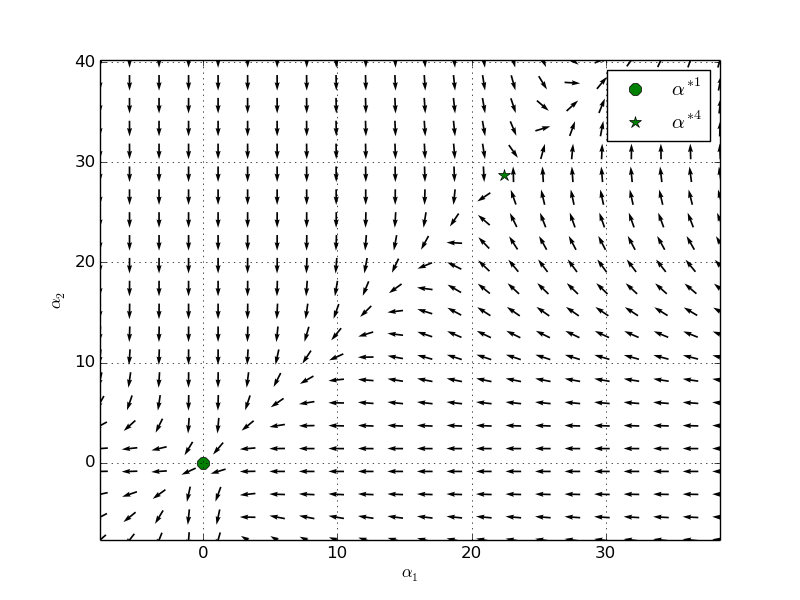
\includegraphics[scale = 0.7]{Python/plots/RG_flow/RG_flow3_2_6_0_2_0_1_0.png}
 \caption{Das Flussdiagramm für eine Lösung vom Typ \ref{Fall1b}. Der Fixpunkt 
  $\alpha^{*}_\text{vw}$ liegt im nicht-perturbativen Bereich. Die Parameter sind 
 $(\Nc,\Nd,\nfc,\nsc,\nfd,\nsd,\nfj,\nsj)=(3,2,6,0,2,0,1,0)$.}
 \label{fig:beta_QCDxdQCD:Sattelpunkt1}
\end{figure}

      
      Der einzige Fall, der in der skalarfreien Theorie physikalische 
      Sattelpunkte bringt, ist \ref{Fall1b}, exemplarisch ist 
      das Flussdiagramm für $\nfj=2$ in Abbildung
      \ref{fig:beta_QCDxdQCD:Sattelpunkt1} zu sehen. Alle drei Fixpunkte 
      liegen, wie in Tabelle \ref{tab:beta_QCDxdQCD:Sattelpunkt} zu sehen, 
      weit im nicht-perturbativen Bereich. Nicht-perturbative 
      $SU(N)$ Dynamiken können in einem Veneziano-limit störungstheoretisch 
      behandelt werden 
      \cite{Jarvinen:2011qe}\cite{Asymptotic_safety_guaranteed}, dabei wird der 
      Grenzfall $N \to \infty , N_\text{f} \to \infty,\nicefrac{N}{N_\text{f}} 
      <\infty,g^2 N\to 0$ betrachtet \cite{VENEZIANO1979213}. Wie im 
      Folgenden gezeigt wird, ist es mit Skalaren jedoch möglich perturbative 
      Fixpunkte zu erhalten, ohne von den Standardmodell Werten $\Nc=3$ und 
      $\nfc=6$ abweichen zu müssen. 
      

      An den Koeffizienten \eqref{eq:beta_QCDxdQCD:X1g} und 
      \eqref{eq:beta_QCDxdQCD:Y1g} sieht man, dass Skalare qualitativ den 
      gleichen Einfluss auf die $\beta$-Funktion wie Fermionen haben, 
      jedoch um einen Faktor $3$-$4$ kleiner, es ist also zu erwarten, dass 
      die Grenzen für die Anzahl der joint-Skalare um einen 
      entsprechenden Faktor höher liegen. Einige mögliche Standardmodell nahe 
      Teilchenzahlen sind in Tabelle 
      \ref{tab:QCDxdQCD:Sattelpunkt_mit_Skalaren} zu sehen. 
      In Abbildung \ref{fig:beta_QCDxdQCD:Fix4_mit_Skalaren} ist außerdem 
      der Fixpunkt $\alpha^{*4}$ für $1\leq \nsd \leq 5$ und sinnvolle $\nsj$ 
      dargestellt. Hier ist zu erkennen, dass $\alpha^{*4}$ betragsmäßtig 
      kleiner wird, je mehr joint-Skalare eingeführt werden.

      \begin{table}
\centering

 \begin{tabular}{ccc|ccc}
 \toprule \midrule
$\Nd$ & $\nsd$ & $\nsj$ &	 $\Nd$ & $\nsd$ & $\nsj$	\\
\midrule
\multirow{5}{*}{2}& $0,1$& $3$-$9$    & \multirow{5}{*}{3} &$0$&$3$\\
 &  $2,3$& $3$-$8$ &  &$1$-$4$&$3,4$\\
 &  $4,5$&$3$-$7$  &  &$5-8$&$2,3,4$\\
 &  $6,7$&$3$-$6$ \\
 &  $8$&$3,4,5$\\    

  \midrule \bottomrule
 \end{tabular}
\caption{Mögliche Anzahlen von Skalaren für $\Nc=3$, $\nfc=6$, $\nfd=0$ .}
\label{tab:QCDxdQCD:Sattelpunkt_mit_Skalaren}
\end{table}

      \begin{figure}[h]
 \centering

 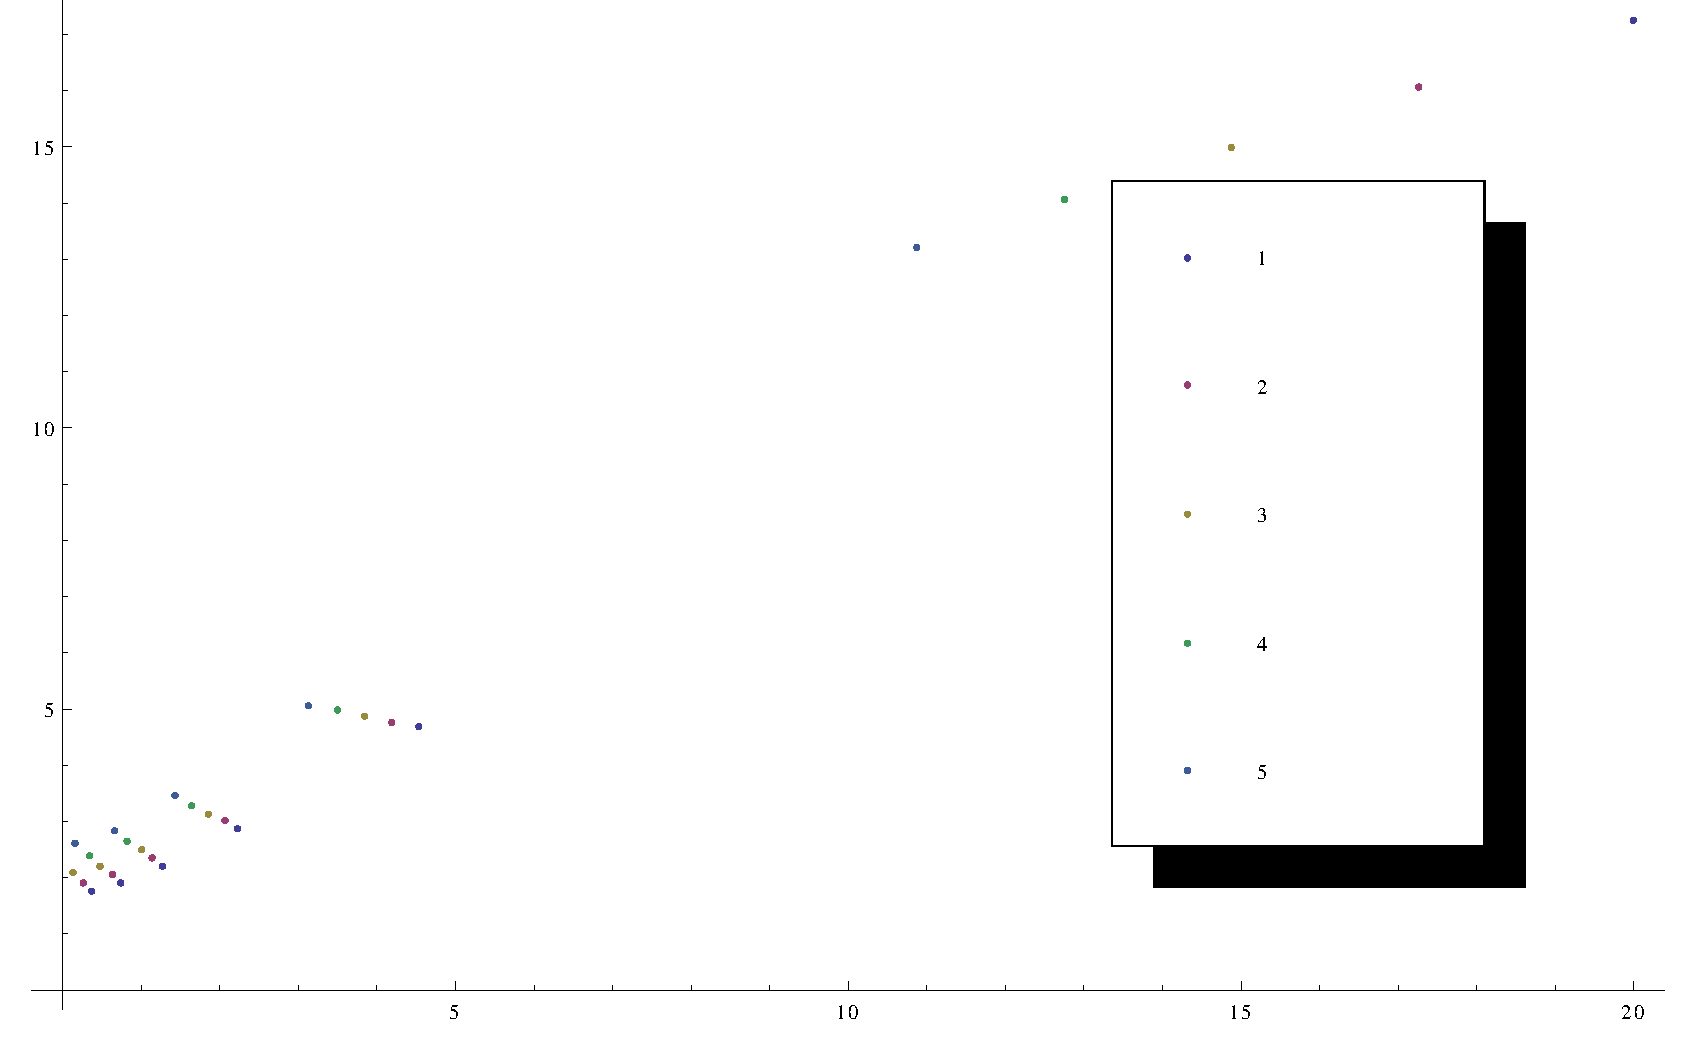
\includegraphics[scale = 0.5]{abschnitte/beta_QCDxdQCD/fig/Fix4_mit_Skalaren.pdf}

 \caption{Lage von $\alpha^{*4}$ in Abhängigkeit von $\nsd$ und $\nsj$.}
 
 \label{fig:beta_QCDxdQCD:Fix4_mit_Skalaren}

 \end{figure}

      
      Um einen vollständig wechselwirkenden UV-Fixpunkt zu erhalten, der mit 
      Methoden der Störungstheorie behandelt werden kann, ist es demnach 
      nötig, skalare Teilchen im joint-Sektor einzuführen. Die Teilchen des 
      dQCD-Sektors haben dagegen, wie in Abbildung 
      \ref{fig:beta_QCDxdQCD:Fix4_mit_Skalaren} zu sehen ist, nur geringe 
      Auswirkungen auf die Lage des Fixpunktes, ob hier Fermionen, Skalare oder 
      beide Teilchensorten eingeführt werden ist qualitativ nicht entscheidend.
      
      
  \subsection{UV-Verhalten bei $\alpha^{*3}$}\label{beta_QCDxdQCD:UV_bei_Fix3}
%     Damit der 
    Da der Fixpunkt $\alpha^{*3}=(-X_1 Y_1^{-1},0)$ ein teilweise 
    wechselwirkender Fixpunkt ist, 
    muss hier das in \ref{beta_im_R2:nicht-hyperbolischer_Fixpunkt} 
    beschriebene Stabilitätskriterium angewendet werden. Zunächst kann aber 
    einfach gezeigt werden, dass dieser Fixpunkt nicht in jede Richtung 
    UV-attraktiv sein kann.
    
    Damit $\alpha^{*3}_1=-X_1 Y_1^{-1} > 0$, muss $X_1<0$ und $Y_1>0$. Es wurde 
    in \ref{beta_QCDxdQCD:fix4:UV} gezeigt, das die umgekehrte Vorzeichenwahl 
    physikalisch nicht sinnvoll ist. Gleichung 
    \eqref{eq:beta_im_R2:stab_matrix_0} zeigt nun 
    $\lambda_1=(\alpha^*_1)^2Y_1 > 0$ zu $e_1=(1,0)^\text{T}$, folglich muss 
    die $\alpha_1$-Achse UV-repulsiv bezüglich $\alpha^{*3}$ sein. 
    
    Am Fixpunkt ergibt sich aus \eqref{eq:beta_im_R2:stab_matrix_0} und 
    \eqref{eq:beta_im_R2:lambda} 
    \begin{equation}
     \lambda_2=0 \quad , \quad  e_2=\begin{pmatrix}
                            -Z_1 Y_1 \\ 1
                           \end{pmatrix}
                           \quad \text{und} \quad
    \quad \nabla \lambda_2 = \begin{pmatrix}
                              0 \\ 2 X_2 -2\frac{X_1}{Y_1} Z_2
                             \end{pmatrix}
                             \quad .
    \end{equation}
    Die Bedingung dafür, dass $\alpha^{*3}$ ein Sattelpunkt ist, ist somit 
    \begin{equation}
     X_1<0 \quad \land \quad Y_1>0 \quad \land \quad X_2 Y_1 < Z_2 X_1
     \quad .
    \end{equation}
    Da die Vorzeichen $X_1<0$, $Y_1>0$ und $X_2<0$ festgelegt sind, 
    kann bereits ohne Fallunterscheidung eine Grenze gefunden werden.
    Aus $X_1<0 \land X_2<0$ folgt allgemein (vgl. \eqref{Fall1b})
	\begin{equation}
	  \left(\nfj+\frac{1}{4} \nsj \right)^2 + \left( \nfj+\frac{1}{4}\nsj 
	  \right) \left( \nfd +\frac14 \nsd \right)\frac1\Nc 
	  + \frac{11}{2} \left(\nfc+\frac14 \nsc \right)\frac1\Nc < 
	  \left( \frac{11}{2} \right)^2 \quad \land \quad \text{c}
	  \leftrightarrow
	  \text{d} \quad. \label{eq:beta_QCDxdQCD:Fix3_ohne_Skalare}
	\end{equation}
   
    Zunächst werden wieder nur Fermionen betrachtet. Da sie außreichen, um 
    perturbative Fixpunkte zu modellieren, wird es nicht nötog sein, Skalare 
    einzuführen.
    Aus 
    \eqref{eq:beta_QCDxdQCD:Fix3_ohne_Skalare} und $X_1<0$ folgen allgemeine 
    Grenzen für $\nfj$, $\Nd$ und $\nfd$
    \begin{equation}
    \begin{aligned}
     &\nfj < \sqrt{\left(\frac{11}{2}\right)^2-\frac{11}{2} \frac{\nfc}{\Nc}}
     =4.39
     \quad , \quad
     \nfd < \left(\left(\frac{11}{2}\right)^2 -1\right) \Nc -\frac{11}{2}
     \nfc = 54.75  \quad ,
     \\
     & \Nd<\frac{11}{2} \Nc -\nfc = 10.5      
    \end{aligned}
    \end{equation}
    für $\Nc=3$ und $\nfc=6$. 
    \begin{table}[h]
\centering
 \begin{tabular}{ccc|c||ccc|c}
 \toprule \midrule
 $\Nd$ 	& $\nfj$ 	& $\nfd$ 	& $\alpha^{*3}_1$ & $\Nd$ 	& $\nfj$ 	& $\nfd$ 	& $\alpha^{*3}_1$		 \\
 \midrule 
 $2$	& $2$		& $0$			& $2.21$  & $6$		& $1$	& $0$-$29$	& $0.75$	\\
 $3$	& $1$		& $0$-$8$		& $5.24$  & $7$		& $1$	& $0$-$35$	& $0.47$	\\
 $3$	& $2$		& $0$-$9$		& $0.85$  & $8$		& $1$	& $0$-$40$	& $0.28$	\\
 $3$	& $3$		& $0$-$7$		& $0.14$  & $9$		& $1$	& $0$-$46$	& $0.14$	\\
 $4$	& $1$		& $0$-$16$		& $2.21$  & $10$	& $1$	& $0$-$51$	& $0.04$	\\
 $4$	& $2$		& $0$-$15$		& $0.28$   		\\
 $5$	& $1$		& $0$-$23$		& $1.23$   		\\
 $5$	& $2$		& $0$-$21$		& $0.04$  		\\
 \midrule \bottomrule
 \end{tabular}
\caption{Mögliche Teilchenzahlen für einen Sattelpunkt bei $\alpha^{*3}$, mit $\Nc=3$, $\nfc=6$ und ohne Skalare.}
\label{tab:beta_QCDxdQCD:Fix3_ohne_Skalare}
\end{table}

    Tabelle \ref{tab:beta_QCDxdQCD:Fix3_ohne_Skalare} zeigt die möglichen 
    Teilchenanzahlen und die Komponente $\alpha^{*3}_1$. Im Gegensatz zum 
    vollständig wechselwirkenden Fixpunkt $\alpha^{*4}$ ist $\alpha^{*3}$ 
    auch für eine Theorie ohne Skalare in einem perturbativ sinnvollen 
    Bereich, demnach können hier zwar wieder Skalare eingeführt werden, 
    ein neues Verhalten oder neue Wertebereiche für den Fixpunkt treten aber 
    nicht auf.
    
    
